\chapter{Experimentos y evaluación}
\label{cap:experimentos}

\section{Implementación del sistema}
Para la implementanción del sistema propuesto, se utilizó como base el motor de procesamiento de \textit{stream} S4 \citep{s4}, cuyo modelo fue explicado en la sección \label{sec:SP}. Para el funcionamiento del sistema de distribución de carga, se desarrolló en Java, donde se incluyó en el código fuente de S4, de esta manera, fue parte del SPS, de tal manera que fuera automático y transparente.

%Dentro del diseño, se propuso un balance de carga según la técnica de replicación, por lo que fue necesario cambiar partes del código fuente de S4. En el Algoritmo \ref{alg:distCarga}
Dado que en el diseño se propuso un balance de carga según la técnica de réplica, fue necesario modificar la forma en que enviaba S4 el flujo a los distintas réplicas del operador. Por lo tanto, lo que se implemento fue un sistema que pudiera escoger la réplica que tuviera menor tamaño en la cola de espera al momento de enviar un dato, de tal manera de escoger siempre al operador con menor carga, y en caso que posean el mismo tamaño, utilizar la primera réplica disponible.

En la Figura \ref{fig:distCarga} se explica gráficamente la distribución de la carga. En la parte (a) el operador A envía un evento al operador B, el cual posee tres réplicas, cuyas menores colas están en la réplica 2 y 3, como son iguales las colas de estas réplicas, se escoge la primera réplica disponible, es decir, la réplica 2. Posteriormente, como la réplica 2 aumento su cola, la réplica 3 es la que posee menor cantidad de cola, como se demuestra en la parte (b), por lo tanto, es la réplica candidata a recibir el dato enviado. Y finalmente, en la parte (c) todas las réplicas posee el mismo tamaño de la cola, por lo tanto, se procede a enviar a la primera réplica.

\begin{figure}[!ht]
	\centering
		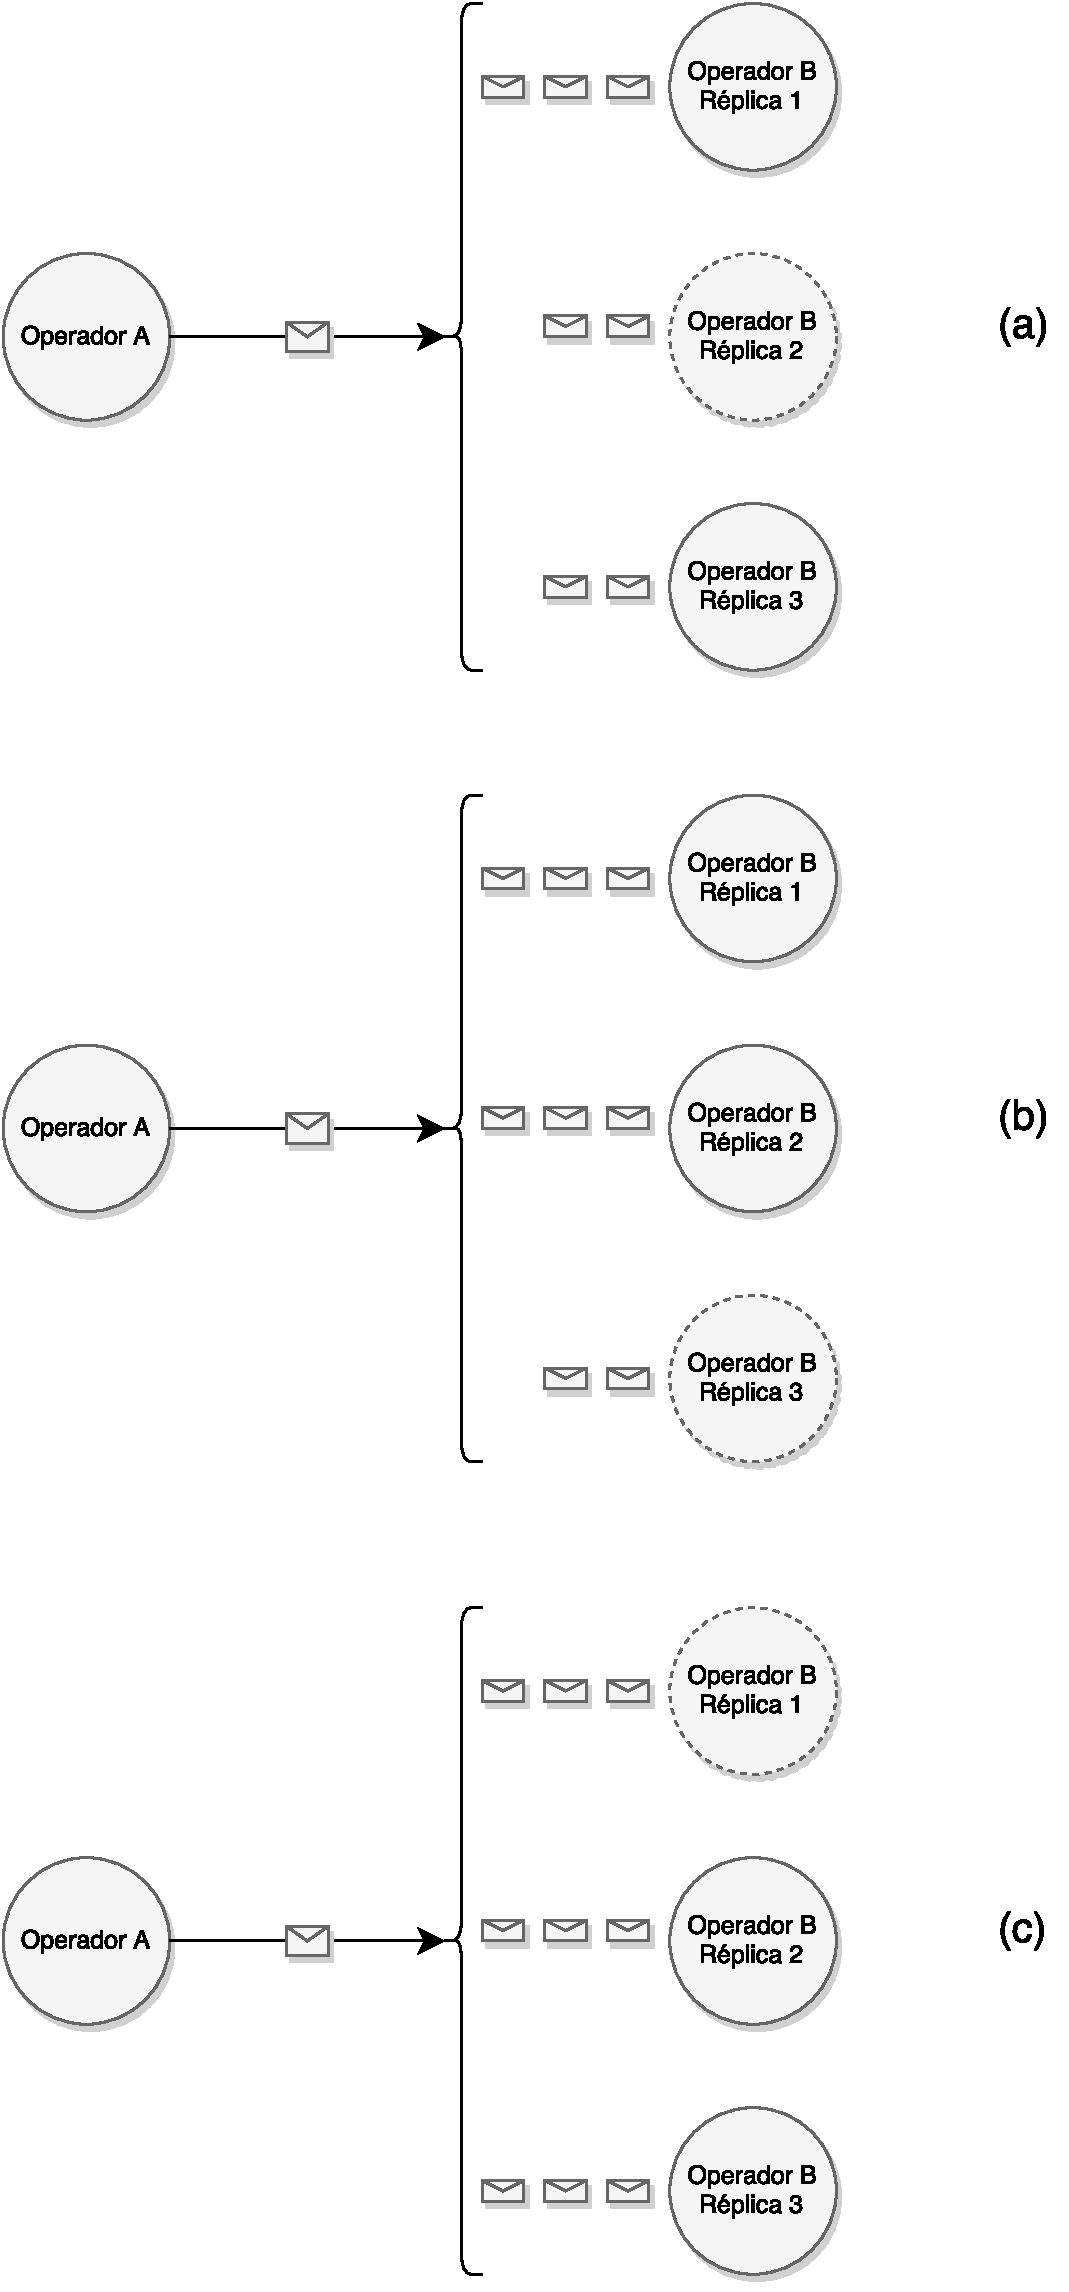
\includegraphics[scale=0.55]{images/DistribucionCarga.pdf}
	\caption{Distribución de la carga entre las réplicas.}
	\label{fig:distCarga}
\end{figure}

En el Algoritmo \ref{alg:distCarga} está descrito la distribución de carga planteada anteriormente, la cual fue implementada en S4 para realizar los experimentos según lo diseñado en el planteamiento de los algoritmos.

\begin{algorithm}[!ht]
	\caption{Distribución de carga entre las réplicas de un operador.}
	\label{alg:distCarga}
	\begin{algorithmic}[1]
	\REQUIRE Evento $\epsilon$ y operador $\phi$.
	\ENSURE Envío del evento a la réplica disponible del operador $\phi$.
	\STATE $\theta \leftarrow minTamanoCola(\phi)$ \COMMENT Se escoge la réplica que posea menor cola
	\STATE $envioEvento(\epsilon,\theta$)
	\end{algorithmic}
\end{algorithm}

Por otra parte, como ya se había mencionado, el sistema de distribución de carga fue parte del código fuente del proyecto de S4. Para el funcionamiento de éste, se procedió a ejecutar dos tareas: enviar las muestras para la historia del operador y enviar las estadísticas del operador, las cuales poseían un intervalo de ejecución de 1 y 5 segundos respectivamente. En el caso del envío de las estadísticas, después de ser enviadas, se consulta el estado de cada uno de los operadores, y en caso de ser necesario, se realiza las modificaci necesarias en el sistema, ya sea de crear o eliminar réplicas de un operador. Los códigos de crear o eliminar replicas se encuentra adjuntos en el Anexo \ref{apendice:codigoFuenteS4}.

Debido al funcionamiento de los SPS, existe una fuente de datos, por lo tanto, para la correcta sincronización de las estadísticas, se procedió a realizar una espera por parte del monitor hasta que la fuente de datos esté lista para enviar los datos. Esta implementanción se puede ver en el Anexo \ref{apendice:codigoFuenteS4}, conjunto con las dos tareas que debe ejecutar después que la fuente de datos avisa de su inicialización.

\section{Experimentos}
Bla bla bla

\subsection{App 1}
Bla bla bla

\subsection{App 2}
Bla bla bla

\subsection{App 3}
Bla bla bla

\section{Evaluación}

Bla bla bla
